\chapter{数学对象与逻辑}
\label{chap:sets-functions-and-proofs}

机器学习中的公式往往把许多计算压缩到一行。例如，要汇总若干样本的预测误差，可以把
各个样本的平方误差相加。这种把有限个数相加的表达式称为有限和：若三个平方误差分别为
$a_1=1$、$a_2=4$和$a_3=9$，则
\[
  \sum_{i=1}^{3}a_i=a_1+a_2+a_3=1+4+9=14.
\]
求和号$\sum$把逐项相加的计算写得更紧凑，下方的$i=1$与上方的$3$说明从第$1$项加到
第$3$项。

给定$n\geq1$个样本
$(\bm{x}_i,y_i)\in\mathbb{R}^d\times\mathbb{R}$，其中$i=1,\ldots,n$，并取
正则化系数$\lambda\geq0$，一个带正则项的最小二乘问题可以写成
\begin{equation}
  \min_{\bm{w}\in\mathbb{R}^d}
  F(\bm{w})
  =
  \frac{1}{2n}\sum_{i=1}^{n}
  \bigl(\bm{w}^{\top}\bm{x}_i-y_i\bigr)^2
  +
  \frac{\lambda}{2}\lVert\bm{w}\rVert_2^2.
  \label{eq:prelim-regularized-least-squares}
\end{equation}
其中$\lambda=0$对应不加正则项的情形。这行公式同时规定了候选参数、样本索引、目标函数和比较准则。若省略
$\bm{w}\in\mathbb{R}^d$，读者便不知道优化在哪个集合上进行；若不说明
$\lambda$的范围，正则项可能鼓励参数变大而不是抑制参数；若把“存在一个参数对所有
样本都预测正确”误写成“对每个样本都存在一个预测正确的参数”，结论甚至会完全改变。

本章把这些容易隐没在公式里的约定展开。集合与关系限定对象的范围，说明怎样分类和比较；
函数与函数族区分输入输出、参数选择以及取值的边界；索引族把对象组织成可以汇总或递推的
形式；命题与证明则写清结论的条件、允许的信息依赖，以及怎样验证这些要求。
这里先建立表达和论证的共同语言。候选数量与程序能力由第~\ref{chap:combinatorics}章
研究，极限和连续变化由第~\ref{chap:mathematical-analysis}章研究。

\section{集合与关系}
\label{sec:prelim-sets-relations-functions}

\subsection{集合运算与结构}

\term{集合}（set）把若干对象作为一个整体讨论。若对象$x$属于集合$X$，记作
$x\in X$；若$X$的每个元素也属于$Y$，记作$X\subseteq Y$。空集记为
$\varnothing$。两个集合的并、交与差分别写作
\[
  X\cup Y,\qquad X\cap Y,\qquad X\setminus Y.
\]
这些运算不仅整理对象，还能表达条件。例如，若$C$是满足资源约束的参数集合，
$D$是使模型有定义的参数集合，那么真正的可行域是$C\cap D$，而不是其中任意一个集合。

集合的描述常有两种方式。列举法直接写出元素，如
$A=\{1,2,3\}$；条件法写成
\[
  A=\{i\in\mathbb{N}:1\leq i\leq 3\}.
\]
冒号右侧是成员必须满足的条件。集合只记录元素是否属于其中，不记录排列顺序，也不重复
计数。因此$\{1,2,3\}$、$\{3,2,1\}$和$\{1,1,2,3\}$表示同一个集合。需要顺序或重复
次数时，应使用序列、多重集合或向量，而不能继续依赖普通集合。

两个集合$X$与$Y$的\term{笛卡尔积}（Cartesian product）是所有有序对组成的集合
\[
  X\times Y=\{(x,y):x\in X,\ y\in Y\}.
\]
“有序”意味着$(x,y)$与$(y,x)$通常不是同一个对象。一个带标签样本可以表示为
$(\bm{x},y)\in\mathbb{R}^d\times\mathbb{R}$；包含$n$个样本的数据集则可以先看成
该集合中的一个长度为$n$的序列。这样写清了一个样本的组成，却还没有对样本怎样产生
作任何概率假设。

集合$X$上的\term{幂集}（power set）$\mathcal{P}(X)$由$X$的全部子集组成。
如果$X=\{a,b\}$，那么
\[
  \mathcal{P}(X)=\{\varnothing,\{a\},\{b\},\{a,b\}\}.
\]
幂集在后文有两类用途。在概率模型中，事件是样本空间$\Omega$的子集；实际允许赋予概率
的事件通常只组成$\mathcal{P}(\Omega)$的一个结构化子族，有限或可数离散样本空间中常取
完整幂集。幂集也可以描述算法可能选择的特征子集或边集合。并非每次出现“若干子集”都
需要完整幂集；允许的子集受到结构限制时，应另写一个集合族。概率事件族需要满足的闭包
条件将在概率论部分说明。

\subsection{关系、等价与分类}

两个对象可以不同，却在当前问题中起同一种作用。例如，不同参数可能给出同一个预测函数，
同一直线上的非零向量也可能表示同一个方向。要把这种“按某种标准视为相同”写清楚，
需要先约定对象之间满足什么关系，再检查该关系能否给出不相交的分类。

集合$X$与$Y$之间的\term{二元关系}（binary relation）是
$X\times Y$的一个子集$R$。写$xRy$表示$(x,y)\in R$。关系允许一个$x$对应多个
$y$，也允许没有对应对象。例如，“不大于”是$\mathbb{R}$上的关系，“样本$i$与样本$j$
之间有边”是索引集合上的关系。

\begin{definition}[等价关系与等价类]
\label{def:prelim-equivalence-relation}
定义在同一个集合$X$上的关系$R$若对任意$x,y,z\in X$满足
\begin{itemize}
  \item 对每个$x\in X$都有$xRx$；
  \item $xRy$蕴含$yRx$；
  \item $xRy$且$yRz$蕴含$xRz$，
\end{itemize}
就称为\term{等价关系}（equivalence relation）。三条性质分别称为自反性、对称性与
传递性。给定$x\in X$，与$x$等价的对象组成它的\term{等价类}（equivalence class）
\[
 [x]_R=\{y\in X:yRx\}.
\]
全部等价类组成的集合记为$X/R$；它们覆盖$X$，且任意两个等价类或者相同，或者不相交。
\end{definition}
例如，在
$\mathbb{R}^2\setminus\{\bm{0}\}$上规定$\bm{x}\sim\bm{y}$当且仅当存在
$c\in\mathbb{R}\setminus\{0\}$使$\bm{x}=c\bm{y}$，那么同一条过原点直线上的非零
向量属于同一个等价类。
后文讨论参数不可识别时，不同参数也可能因为产生同一个可观测对象而落入同一等价类。

分类关心哪些对象可以合并，比较优劣则关心对象能否排在另一个对象之前。这是另一种关系，
不能把它与等价关系混用。
\begin{definition}[偏序关系]
\label{def:prelim-partial-order}
集合$X$上的\term{偏序关系}（partial order）$R$对任意$x,y,z\in X$满足自反性
$xRx$、传递性，以及反对称性：$xRy$且$yRx$时必须有$x=y$。
若任意两个元素还至少满足$xRy$或$yRx$中的一个，则称为全序。
\end{definition}
集合包含关系$\subseteq$就是偏序。偏序中的两个元素
未必可比较，例如$\{1\}$和$\{2\}$都不是对方的子集。这一点会在多目标优化中再次出现：
两个方案可能各自在一个目标上更好，因而不能排成一条总的优劣顺序。

\section{函数、函数族与取值范围}
\label{sec:prelim-functions-value-ranges}

关系可以记录多种配对，函数则要求每个输入有唯一输出。以下先说明一次映射的取值与组合，
再比较参数化得到的整族函数，以及实值函数能够取得或接近哪些数值。

\subsection{函数的取值范围与逆映射}

\term{函数}（function）$f:X\to Y$为每个$x\in X$指定唯一的$f(x)\in Y$。
$X$称为定义域，$Y$称为陪域。函数在定义域上的实际输出组成
\[
  f(X)=\{f(x):x\in X\},
\]
称为像。陪域是函数定义的一部分，像则由函数实际取到的值决定，二者不必相等。
例如$f:\mathbb{R}\to\mathbb{R}$、$f(x)=x^2$的像是$[0,\infty)$。
给定$B\subseteq Y$，集合
\[
  f^{-1}(B)=\{x\in X:f(x)\in B\}
\]
称为$B$在$f$下的\term{原像}（preimage）。这里的$f^{-1}(B)$只表示满足输出条件的
输入集合，即使$f$没有逆函数也有定义；它不能与后文双射的逆函数混为一谈。

函数$f:X\to Y$若满足$f(x_1)=f(x_2)$必然推出$x_1=x_2$，就称为
\term{单射}（injective function）；它不会把两个不同输入压成同一个输出。若每个
$y\in Y$都能写成$f(x)$，就称为\term{满射}（surjective function）；它覆盖整个陪域。
同时为单射和满射的函数称为双射。只有双射才存在定义在整个$Y$上的逆函数
$f^{-1}:Y\to X$，并满足
\[
  f^{-1}(f(x))=x,\qquad f(f^{-1}(y))=y.
\]
若$f$只是单射，可以在像$f(X)$上定义逆；若$f$不是单射，同一个输出对应多个输入，
所谓“反求参数”便需要额外约束或只能返回一个集合。

\subsection{复合映射与输入输出匹配}

若计算分成多个变换，后一个变换必须能接收前一个变换的输出。函数复合把这项兼容条件
与具体求值次序同时写进表达式。
给定$f:X\to Y$与$g:Y\to Z$，它们的\term{复合}（composition）是
\[
  (g\circ f)(x)=g(f(x)).
\]
复合次序不能任意交换，因为$g\circ f$与$f\circ g$的定义域可能不同，即使都能定义，
结果也通常不同。机器学习模型常由多层变换复合而成；检查每层输入输出的集合或维度，
是发现公式错误的一种直接方法。
再给定$h:Z\to U$，复合满足结合律：
\[
  h\circ(g\circ f)=(h\circ g)\circ f.
\]
恒等映射$\operatorname{id}_X(x)=x$不改变输入，并满足
$f\circ\operatorname{id}_X=f$与$\operatorname{id}_Y\circ f=f$。若$f$与$g$均为
双射，则$g\circ f$也是双射，且$(g\circ f)^{-1}=f^{-1}\circ g^{-1}$；逆映射的次序
与原复合次序相反。

\subsection{函数参数化与可识别性}

前面把输入送入一个固定函数；选择模型时则要在一组函数中挑选一个对象。
必须区分函数$f$、输入$x$与函数值$f(x)$。式
\eqref{eq:prelim-regularized-least-squares}中的$F$是把每个参数向量映射到一个实数的
函数，$F(\bm{w})$才是参数$\bm{w}$对应的目标值。若要讨论一组候选函数，应把它们写成
函数集合，例如
\[
  f_{\bm{w}}:\mathbb{R}^d\to\mathbb{R},
  \qquad
  f_{\bm{w}}(\bm{x})=\bm{w}^{\top}\bm{x},
  \qquad
  \mathcal{F}=\{f_{\bm{w}}:\bm{w}\in\mathbb{R}^d\}.
\]
这里$\bm{w}$索引函数，$\bm{x}$是函数的输入。混淆这两个角色，会使“优化参数”和
“对新输入求值”看起来像同一步操作。
更准确地说，参数化给出了映射$\bm{w}\mapsto f_{\bm{w}}$。它的输入是参数向量，输出
却是一个函数，而不是这个函数在某个固定输入上的函数值；这里的函数值是标量。这个映射
若不是单射，不同参数就会表示同一个函数；因此参数集合与由它表示的函数集合也不能直接
视为同一个集合。

\begin{definition}[函数参数化的可识别性]
\label{def:prelim-identifiable-parameterization}
给定参数集合$\Theta$与函数族$\{f_\theta:X\to Y:\theta\in\Theta\}$。
若$f_\theta=f_{\theta'}$蕴含$\theta=\theta'$，即$\theta\mapsto f_\theta$为单射，
则称这一函数参数化可识别；否则称为不可识别。
\end{definition}
这里的相等比较整个定义域上的函数。若只观察部分输入，即使整个函数族的参数化可识别，
这部分观测也可能不足以辨认参数。

\begin{example}[参数不同而函数相同]
\label{ex:prelim-nonidentifiable-parameterization}
考虑参数化函数
\[
  f_{a,b}:\mathbb{R}\to\mathbb{R},
  \qquad
  f_{a,b}(x)=abx,
  \qquad
  (a,b)\in\mathbb{R}^2.
\]
参数$(1,2)$与$(2,1)$不同，却对每个$x$给出相同的函数值。更一般地，只要$c\neq0$，
$(ca,b/c)$与$(a,b)$表示同一个函数。由于定义域包含非零输入，例如取$x=1$，从完整的
输入输出关系可以确定乘积$ab$，却不能分别确定$a$和$b$。这是参数化的不可识别性，而
不是计算精度不足。
\end{example}

\subsection{实值函数的界与极值}
\label{sec:prelim-optimal-values-errors}

比较函数值之前，需要区分它们能够接近的边界和实际取得的数值。
对非空实数集合$A$，若数$b$不大于$A$的每个成员，就称$b$为它的下界；上界的方向相反。
最小元素必须属于$A$，下确界则只要求是全部下界中最大的一个。
下面把这个区别用于实值函数的像集$A=f(X)$，并区分最佳数值与达到它的输入。


设$X$非空且$f:X\to\mathbb{R}$。若$x^\star\in X$满足
\[
  \forall x\in X,\qquad f(x^\star)\leq f(x),
\]
则$x^\star$是一个\term{全局最小点}（global minimizer），$f(x^\star)$是最小值。
所有最小点组成集合
\[
  \argmin_{x\in X} f(x)
  =\{x\in X:\forall z\in X,\ f(x)\leq f(z)\}.
\]
有最小值时，这也等于$\{x\in X:f(x)=\min_{z\in X}f(z)\}$。
$\argmin$返回输入的集合，而$\min$返回数值；多个输入可以取得同一个最小值。
如果没有输入取得最佳数值，就没有最小点，最小点集合为空。

即使没有最小值，只要$f(X)$有下界，仍可定义\term{下确界}（infimum）
\[
  f^\star=\inf_{x\in X}f(x).
\]
$f^\star$是$f(X)$的最大下界：每个$f(x)$都不小于$f^\star$，并且任何更大的数都不再
是下界。例如$f(x)=x$、$X=(0,1)$满足$\inf_{x\in X}f(x)=0$，但不存在
$x\in X$使$f(x)=0$。

与下界对称，若$f(X)$有上界，则它的最小上界称为\term{上确界}（supremum），记为
\[
  \sup_{x\in X}f(x).
\]
若某个$x^\star\in X$达到这个数值，便得到最大值和最大点。所有最大点组成
$\argmax_{x\in X}f(x)$；有最大值时，
\[
  \argmax_{x\in X}f(x)
  =\{x\in X:f(x)=\max_{z\in X}f(z)\}.
\]
它与$\argmin$一样返回输入集合，没有最大点时该集合为空。下确界、上确界描述可逼近
的边界，最小值、最大值则额外要求边界由定义域中的元素达到。若$f$无下界，约定
$\inf_{x\in X}f(x)=-\infty$；若$f$无上界，则相应上确界为$+\infty$。

图~\ref{fig:prelim-minimum-infimum}固定同一个函数$f(x)=x$，只改变定义域是否包含端点。
两侧的函数值都以$0$为下确界；右侧把$x=0$纳入定义域后，这个下确界才由某个输入达到。
比较的关键是边界点是否属于定义域，而不是两条曲线是否趋向同一个高度。

\begin{figure}[htbp]
  \centering
  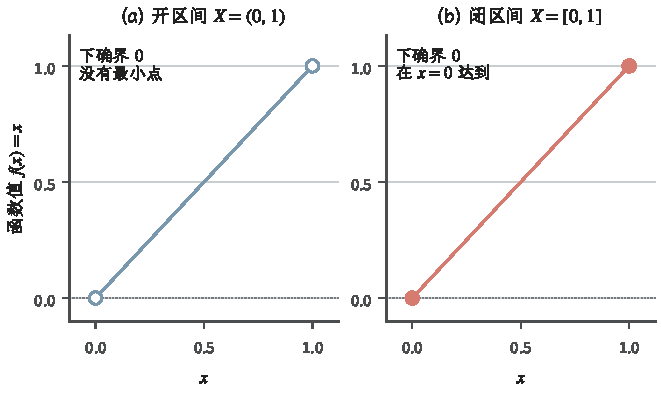
\includegraphics[width=\linewidth]{figures/math-preparation/analysis-concepts/language-minimum-infimum.pdf}
  \caption{同一函数$f(x)=x$的边界对照。左图定义域为$(0,1)$，空心端点不属于图像，函数值可任意接近$0$，却不能取到；右图定义域为$[0,1]$，实心端点$(0,0)$达到下确界。两图的下确界相同，最小点是否存在取决于可行端点是否保留。图为解析教学示例。}
  \label{fig:prelim-minimum-infimum}
\end{figure}

\section{索引族的汇总与递推}
\label{sec:prelim-indices-sums-recurrences}

\subsection{索引族、有限序列与数列}

函数可以把每个索引对应到一个对象，从而保留对象的编号与重复出现。
\begin{definition}[索引族]
\label{def:prelim-indexed-family}
给定索引集合$I$和对象集合$X$，一个索引族是映射$a:I\to X$。
通常把$a(i)$写作$a_i$，整个族写作$(a_i)_{i\in I}$。
\end{definition}
当$I=\{1,\ldots,n\}$并按整数顺序读取时，得到有限序列；当$I$为正整数集时，得到
无限序列，取值为实数时通常称为数列。二维数组则使用索引对$(i,j)$。
索引族允许不同索引对应同一对象，而集合只保留对象是否出现；两者因此不能互相替代。
下面只研究怎样取出、汇总和递推这些对象，数列极限留待分析章。

\subsubsection{索引角色与取值范围}

索引把一族对象排成可引用的形式。本书通常用$i,j,k$标识元素或样本，用$n$表示样本数，
用$d$表示特征维数，用带括号的上标$t$表示迭代步。例如，
$\bm{x}_i\in\mathbb{R}^d$是第$i$个样本，
$x_{i,j}$是该样本的第$j$个坐标，
$\bm{w}^{(t)}$是第$t$次迭代的参数。普通上标则保留给幂：
$w_j^2$表示平方，而$w_j^{(2)}$表示第$2$次迭代中的第$j$个坐标。
若对象本身按时间排列，还应另行声明时间下标，例如$\bm{z}_{\tau}$表示时刻$\tau$的
状态。样本编号、物理时间和算法迭代都可以取整数值，但它们索引的是不同对象，不能仅因
数值相同就互换。

下标只有在取值范围明确时才有意义。把章首的三项有限和推广到$n$项，其中$n$为正整数，得到
\[
  \sum_{i=1}^{n}a_i=a_1+a_2+\cdots+a_n.
\]
其中$i$是求和过程中变化的\term{哑索引}
（dummy index）。把$i$换成$k$不会改变结果。与之不同，等式
\[
  b_j=\sum_{i=1}^{n}x_{i,j}
\]
中的$j$是自由索引：等式对哪些$j$成立需要在附近说明，而且改变$j$会选取不同坐标。
同一个符号不能在一项中既作哑索引又作自由索引。

双重求和需要同时写清两个范围。对有限数组$a_{i,j}$，
\[
  \sum_{i=1}^{n}\sum_{j=1}^{d}a_{i,j}
  =
  \sum_{j=1}^{d}\sum_{i=1}^{n}a_{i,j},
\]
因为两边都遍历同一个有限索引集
$\{1,\ldots,n\}\times\{1,\ldots,d\}$，并把每个索引对$(i,j)$对应的项$a_{i,j}$
恰好相加一次。后文把有限和换成无限级数或积分时，交换次序将需要额外条件，不能直接沿用
这个有限情形的结论。

\subsection{有限和、乘积与加权平均}

有限和中的各项可以先乘系数再相加，也可以先分别求和再乘系数。这来自加法与乘法的
分配律，称为求和的线性关系。对标量$a,b$与同长度序列$(u_i)$、$(v_i)$，
\[
  \sum_{i=1}^{n}(au_i+bv_i)
  =
  a\sum_{i=1}^{n}u_i+b\sum_{i=1}^{n}v_i.
\]
若权重$\alpha_i\geq0$且$\sum_{i=1}^{n}\alpha_i=1$，则
$\sum_i\alpha_i u_i$称为有限\term{加权平均}（weighted average）。
普通样本平均对应$\alpha_i=1/n$。这个简单对象会成为积分与期望的有限版本：积分允许
位置形成连续集合，期望则按概率分配权重。
例如，章首三个平方误差的普通平均是$(1+4+9)/3=14/3$；若权重改为
$1/2$、$1/4$、$1/4$，则加权平均是
$\frac12\cdot1+\frac14\cdot4+\frac14\cdot9=15/4$。两者使用同一组数值，改变的是各项
在汇总结果中的权重。

有限乘积写作$\prod_{i=1}^{n}a_i$。按照空操作不改变结果的约定，
\[
  \sum_{i\in\varnothing}a_i=0,\qquad
  \prod_{i\in\varnothing}a_i=1.
\]
这两个约定分别把$0$和$1$作为加法与乘法的单位元，使递推公式在边界处仍可保持统一。
使用乘积前仍应检查零因子与符号；对正数取对数可把乘积变成和，但含零或负数时不能直接
这样做。

\subsection{递推关系与状态更新}

有限和也可以随着数据到来逐步计算。例如，三个平方误差$1$、$4$、$9$依次到达时，
不必每收到一项就把已有各项重新相加。记$S^{(t)}$为收到前$t$项后的累计值，只需保存
上一轮的累计值，并把新到的一项加进去：
\[
  S^{(0)}=0,\qquad S^{(t+1)}=S^{(t)}+a_{t+1},\qquad t=0,1,2.
\]
在这个例子中，更新依次给出$S^{(1)}=1$、$S^{(2)}=5$、$S^{(3)}=14$。第$t+1$轮只需
知道$S^{(t)}$和新值$a_{t+1}$，而不必保存前$t$项；展开更新则回到
$S^{(t)}=\sum_{i=1}^{t}a_i$。有限和写出累计结果，更新规则写出怎样逐步得到这个结果。

这种从初值出发，用已有项确定后续项的关系称为\term{递推}（recurrence）。对这样的逐步
求值规则，更新规则与初值共同确定序列，只有更新规则通常不能确定每一项。递推也不一定
累加数值：若某种修正
每轮把当前偏差缩小一半，从偏差$8$出发便依次得到$4$、$2$、$1$。用$e^{(t)}$表示
第$t$轮的带符号偏差，把$1/2$推广为固定系数$\rho\in\mathbb{R}$，可写成
\begin{equation}
  e^{(t+1)}=\rho e^{(t)},\qquad e^{(0)}=e_0,\qquad t=0,1,\ldots,
  \label{eq:prelim-geometric-recurrence}
\end{equation}
对整数$t\geq1$逐步展开得到
\[
  e^{(t)}=\rho^t e_0.
\]
对非零初始偏差，$|\rho|<1$使每一步的绝对值缩小，$\rho=-1$使大小不变而符号交替，
$|\rho|>1$使它放大。若$e_0=0$，每一项都是零。这里先由更新规则确定有限步结果；
这些结果在无限多步之后怎样变化，将在分析章讨论。

更一般的误差递推
\begin{equation}
  e^{(t+1)}\leq \rho e^{(t)}+\delta_t,
  \qquad 0\leq\rho<1,
  \label{eq:prelim-perturbed-recurrence}
\end{equation}
包含每一步新加入的非负扰动$\delta_t$，这里将$e^{(t)}$视为非负误差。这个不等式只给出
下一步的误差上界，而不指定它的精确值。再次使用递推不等式，
并利用$\rho\geq0$使不等号方向保持不变，得到
\[
  \begin{aligned}
    e^{(2)}&\leq\rho^2e^{(0)}+\rho\delta_0+\delta_1,\\
    e^{(3)}&\leq\rho^3e^{(0)}+\rho^2\delta_0+\rho\delta_1+\delta_2.
  \end{aligned}
\]
新扰动加入时权重为$1$，此后每经过一轮就再乘一次$\rho$。把这组逐项相加的表达式写成
有限和，对整数$t\geq1$展开$t$步可得
\begin{equation}
  e^{(t)}
  \leq
  \rho^t e^{(0)}
  +
  \sum_{s=0}^{t-1}\rho^{t-1-s}\delta_s.
  \label{eq:prelim-unrolled-recurrence}
\end{equation}
第一项记录初始误差在$t$步后的权重，第二项汇总前$t$步新加入的扰动。
新加入的项经过的更新次数不同，权重也不同；这个有限展开还没有对无限步极限作保证。

式~\eqref{eq:prelim-unrolled-recurrence}可以用数学归纳法证明：先核对$t=1$的基例，再
假设结论对$t$成立并据此推出$t+1$时的结论。完整证明将在本章介绍归纳法时给出。

\section{命题与证明}
\label{sec:prelim-propositions-quantifiers}

对象和计算规则写清之后，还需说明声称了什么：条件在哪些对象上成立，一个选择能依赖
哪些信息，结论要求存在还是唯一。逻辑把这些要求写成真假条件明确的陈述，证明则说明它们
为何由已给条件推出。

\subsection{命题、量词与依赖关系}

\subsubsection{命题与逻辑运算}

\term{命题}（proposition）是在给定语境中具有真假值的陈述。“$F$有最小值”是命题，
“求$F$的最小值”则是任务。带变量的表达式如“$x^2\geq0$”还需要说明$x$的取值范围
或添加量词，才成为完整命题。对实数它成立，对复数若使用通常的序关系则没有定义。

命题$P$的否定记为$\neg P$。两个命题的“且”“或”分别记为
$P\land Q$和$P\lor Q$。数学中的“或”通常是可兼容的：$P$和$Q$同时为真时，
$P\lor Q$仍为真。若只允许恰有一个成立，需要明确写成异或条件。

\term{蕴含}（implication）$P\Rightarrow Q$表示只要$P$为真，$Q$就必须为真。
这里$P$是$Q$的充分条件，$Q$是$P$的必要条件。反向命题$Q\Rightarrow P$需要单独
证明。两向都成立时写作$P\Leftrightarrow Q$，称为等价条件。

定理中的假设正是在限定$P$所覆盖的对象。例如，“目标函数连续且可行域紧致”只允许把
结论用于同时满足这两个条件的问题，不能从定理名称中删去其中一个条件。类似地，“存在
一个最优解”是$\exists x^\star\in X$开头的命题，而“每个初值产生的迭代都收敛”是
$\forall x^{(0)}\in X$开头的另一命题；前者成立并不自动给出后者。

以实数$x$为例，$x>1$是$x^2>1$的充分条件，却不是必要条件，因为$x<-1$时也有
$x^2>1$。条件$x\neq0$是$x^2>0$的充分必要条件。把充分条件误当作必要条件，会排除
本来可能成立的情形；把必要条件误当作充分条件，则可能把不合格对象当成解。

\subsubsection{全称量词与存在量词}

\term{全称量词}（universal quantifier）$\forall$表示“对每一个”，
\term{存在量词}（existential quantifier）$\exists$表示“至少存在一个”。例如
\[
  \forall x\in\mathbb{R},\quad x^2\geq0
\]
是全称命题，而
\[
  \exists x\in\mathbb{R},\quad x^2=2
\]
是存在命题。存在并不表示唯一；要表达恰有一个对象满足条件，可以写
$\exists!x$，但使用时仍应说明存在性与唯一性各由什么保证。

否定量词时，量词种类与内部命题同时改变：
\begin{align*}
  \neg\bigl(\forall x\in X,\ P(x)\bigr)
  &\Longleftrightarrow
  \exists x\in X,\ \neg P(x),\\
  \neg\bigl(\exists x\in X,\ P(x)\bigr)
  &\Longleftrightarrow
  \forall x\in X,\ \neg P(x).
\end{align*}
所以，要推翻“每个输入都满足性质$P$”，找到一个不满足的输入即可；要证明“没有输入
满足$P$”，则必须排除所有输入。

\subsubsection{量词次序与依赖关系}

考虑样本集合$S=\{1,\ldots,n\}$和参数集合$W$，令$C(w,i)$表示参数$w$在第$i$个
样本上预测正确。陈述
\begin{equation}
  \exists w\in W,\quad \forall i\in S,\quad C(w,i)
  \label{eq:prelim-one-parameter-all-samples}
\end{equation}
要求找到同一个参数，使它对所有样本都正确。陈述
\begin{equation}
  \forall i\in S,\quad \exists w\in W,\quad C(w,i)
  \label{eq:prelim-each-sample-some-parameter}
\end{equation}
却允许参数随样本改变，因而弱得多。

\begin{example}[逐点可选不等于统一可选]
\label{ex:prelim-quantifier-order}
令$S=W=\{0,1\}$，并规定$C(w,i)$当且仅当$w=i$。对每个$i$，选择$w=i$即可，
所以式~\eqref{eq:prelim-each-sample-some-parameter}成立。但不存在一个$w$同时等于
$0$和$1$，所以式~\eqref{eq:prelim-one-parameter-all-samples}不成立。
\end{example}

\begin{table}[htbp]
 \centering\small
 \begin{tabularx}{\linewidth}{@{}lccX@{}}
 \toprule
 参数 & 样本$0$ & 样本$1$ & 对量词的含义\\
 \midrule
 $w=0$ & 成立 & 不成立 & 不能覆盖全部样本\\
 $w=1$ & 不成立 & 成立 & 不能覆盖全部样本\\
 \bottomrule
 \end{tabularx}
 \caption{例~\ref{ex:prelim-quantifier-order}的条件真值。每一列都有一个可选参数，却没有一行同时成立。}
 \label{tab:prelim-quantifier-truth-pattern}
\end{table}

例~\ref{ex:prelim-quantifier-order}说明，量词次序改变了允许依赖哪些信息。
统计学习中的“对每个允许分布，以高概率得到小误差”也包含多个量词；算法、样本量和
失败概率是否可以依赖分布，必须由量词位置决定，不能靠自然语言猜测。

\subsection{公式模型与逻辑后承}

\subsubsection{赋值、子句与满足}


把逻辑连接词作用于有限个命题变量，便得到\term{布尔公式}（Boolean formula）。
变量各取什么值是一件事，整个公式是否成立是另一件事；为了检验规则，需要把这两层对象
明确区分。蕴含也可以写成一个不允许反例的析取式：
\begin{equation}
  P\Rightarrow Q\quad\Longleftrightarrow\quad\neg P\lor Q.
  \label{eq:comb-implication-clause}
\end{equation}

\begin{definition}[赋值与公式的模型]
\label{def:comb-assignment-model}
给定命题变量$z_1,\ldots,z_n$，\term{赋值}（assignment）是映射
$\nu:\{z_1,\ldots,z_n\}\to\{\mathrm{false},\mathrm{true}\}$；连接词的真值规则
递归地确定$\nu$是否满足一个公式。满足公式$\Phi$的赋值也称为$\Phi$的
\term{模型}（model），全体模型记为$\operatorname{Mod}(\Phi)$。
\end{definition}
这个“模型”只指
逻辑公式的满足赋值，不等同于后续章节中由参数描述的统计模型。

否定复合命题时，De Morgan律给出
\begin{equation}
  \neg(P\land Q)\Longleftrightarrow(\neg P\lor\neg Q),
  \qquad
  \neg(P\lor Q)\Longleftrightarrow(\neg P\land\neg Q).
  \label{eq:comb-de-morgan}
\end{equation}
以第一式为例，$(P,Q)$依次取$(0,0),(0,1),(1,0),(1,1)$时，等式两侧的真值都依次为
$1,1,1,0$；第二式同理得到$1,0,0,0$。逐行相同证明两边具有相同模型集合，而不是
仅在某个选定赋值上碰巧相等。

为把多条规则写在一起，需要区分规则中的基本真假项与一条完整要求。
\begin{definition}[文字、子句与合取范式]
\label{def:comb-literals-cnf}
一个文字是命题变量$z_i$或它的否定$\neg z_i$；一个子句是若干文字的析取，
只要其中至少一个文字为真，该子句就为真。若公式由若干子句合取而成，就称为
\term{合取范式}（conjunctive normal form, CNF），它要求所有子句同时为真。
\end{definition}

取四个候选$V_0=\{1,2,3,4\}$，用$z_i$表示“候选$i$被选择”，真与假分别记作$1$与$0$。
要求候选$1$与$2$恰选一个，候选$3$被选时必须选$1$，候选$4$被选时必须选$2$或$3$。
这些规则可以写成
\begin{equation}
  \Phi(\bm{z})
  =
  (z_1\lor z_2)
  \land(\neg z_1\lor\neg z_2)
  \land(\neg z_3\lor z_1)
  \land(\neg z_4\lor z_2\lor z_3).
  \label{eq:comb-running-cnf}
\end{equation}
前两个子句共同表达$z_1,z_2$恰有一个为真；第三个子句表达
$z_3\Rightarrow z_1$；第四个子句表达$z_4\Rightarrow(z_2\lor z_3)$。


\begin{definition}[满足、可满足与永真]
\label{def:comb-satisfiability}
赋值$\bm{z}$若使$\Phi(\bm{z})$为真，就称它\term{满足}（satisfy）$\Phi$。
至少存在一个满足赋值时，公式\term{可满足}（satisfiable）；不存在时称为不可满足。
这里要判断的是
\[
  \exists\bm{z}\in\{0,1\}^n,\quad \Phi(\bm{z})=\mathrm{true},
\]
不是证明$\Phi$对每个赋值都真。对每个赋值都真的公式称为永真式；可满足性与永真性
对应不同的量词，不能混用。
\end{definition}

例如，赋值$(1,0,0,0)$与$(0,1,0,1)$都满足这组规则，
$(1,1,0,0)$却违反前两个候选的互斥要求。第~\ref{chap:combinatorics}章将把模型
写成候选集合，研究模型数量、寻找模型的程序及其代价；这里先检验陈述的真假含义。

\subsubsection{后承、多个模型与冲突}

一个可行答案只说明一组规则不矛盾；要判断另一条结论是否被规则强制，还需检查所有可行答案。
\begin{definition}[逻辑后承]
\label{def:comb-logical-consequence}
若每个满足$\Phi$的赋值也满足命题$\Psi$，记作
\[
  \Phi\models\Psi,
\]
称$\Psi$是$\Phi$的\term{逻辑后承}（logical consequence）。
\end{definition}
这表示规则已经强制
推出$\Psi$，不表示某个求解器碰巧返回了满足$\Psi$的一个答案。例如，由
式~\eqref{eq:comb-running-cnf}可得
\[
  \Phi\models(z_3\Rightarrow\neg z_2),
\]
因为$z_3$推出$z_1$，而$z_1$与$z_2$互斥。还可得
\[
  \Phi\land z_4\land\neg z_2
  \models z_3\land z_1.
\]
后一结论使用了额外观测$z_4=1,z_2=0$，不能去掉这些条件后仍声称
$\Phi\models z_3$。用真变量的下标集合表示一个模型，$\Phi\land z_4\land\neg z_2$只有
$\{1,3,4\}$这一个模型；原公式$\Phi$则有五个模型。这组规则因此同时给出了唯一答案、
多个答案与下段冲突情形的可复核对照。

规则允许多个模型时，可满足性只确认“至少有一个答案”。$\{1\}$与$\{2,4\}$都满足
$\Phi$，所以规则本身没有在二者之间作出选择。若再加入$z_2$与$z_3$这两个只含一个文字的单位子句，
公式变为不可满足：$z_3$推出$z_1$，却又要求互斥的$z_2$为真。冲突表示全部硬规则
无法同时成立，不等于程序尚未找到答案。

判断$\Phi\models\Psi$可以转化为一次不可满足性检查：
\begin{equation}
  \Phi\models\Psi
  \quad\Longleftrightarrow\quad
  \Phi\land\neg\Psi\text{ 不可满足}.
  \label{eq:comb-entailment-unsat}
\end{equation}
若右侧可满足，其模型就是一个满足$\Phi$却违反$\Psi$的反例；若右侧不可满足，
这样的反例不存在。这个等价关系把全称式的逻辑后承转换为存在反例的搜索。

定义还包含一个容易误读的边界：若$\Phi$本身不可满足，则
$\operatorname{Mod}(\Phi)=\varnothing$，因而对任意$\Psi$都有
$\Phi\models\Psi$。这称为空真，并不表示冲突规则提供了关于$\Psi$的有效信息。
实际推理通常先检查$\Phi$可满足，再解释它的逻辑后承。

\subsection{证明形式与合法反例}
\label{sec:prelim-proofs-constructions-counterexamples}

同一个结论可以用不同方式论证，选择哪一种取决于已知条件能怎样发挥作用。本节用几个
短例子比较这些方式：蕴含命题可以从条件推到结论，也可以排除结论不成立的情形；存在
命题可以给出满足条件的对象；由整数索引的一族命题则可以利用相邻项之间的递推关系。
反例承担另一项任务：找出一个满足前提却违反结论的对象，以说明某个全称命题不成立。

\subsubsection{直接证明、逆否证明与反证法}

证明不是把若干正确公式排列在一起，而是从已给条件出发，经过每一步都合法的推理到达
结论。开始证明前，先辨认命题的逻辑形式。对$P\Rightarrow Q$，直接证明从$P$出发；
逆否证明改证$\neg Q\Rightarrow\neg P$；反证法假设$P$成立而$Q$不成立，并推出矛盾。
这些形式在逻辑上等价，但哪一种更清楚取决于条件怎样进入计算\scite{math-graham1994concrete}

下面用最小点的唯一性说明反证法怎样工作。最小点是允许范围内没有更小函数值的点；要
排除两个不同的最小点，可以反设它们存在，再构造一个函数值更小的允许点。

\begin{example}[用反证法排除两个最小点]
\label{ex:prelim-strict-midpoint-unique-minimizer}
设$C\subseteq\mathbb{R}^d$满足：任取$\bm{u},\bm{v}\in C$，其中点
$(\bm{u}+\bm{v})/2$仍属于$C$。若函数$F:C\to\mathbb{R}$对任意不同的
$\bm{u},\bm{v}\in C$都满足
\begin{equation}
  F\left(\frac{\bm{u}+\bm{v}}{2}\right)
  <
  \frac{F(\bm{u})+F(\bm{v})}{2},
  \label{eq:prelim-strict-midpoint-condition}
\end{equation}
那么$F$在$C$上至多有一个最小点。

中点条件提供了构造更小函数值的办法。反设
$\bm{u}\neq\bm{v}$都是最小点，并把共同的最小值记为$m$。由$C$对取中点封闭，
$(\bm{u}+\bm{v})/2\in C$。再由式~\eqref{eq:prelim-strict-midpoint-condition}，
\[
  F\left(\frac{\bm{u}+\bm{v}}{2}\right)
  <
  \frac{m+m}{2}
  =m.
\]
这与$m$是最小值矛盾，所以不可能存在两个不同的最小点。
例如，$F(x)=x^2$在$\mathbb{R}$上满足这一条件，因为
\[
  \frac{u^2+v^2}{2}-\left(\frac{u+v}{2}\right)^2
  =\frac{(u-v)^2}{4}>0\qquad(u\neq v).
\]
这里不是逐个检查所有候选点，而是说明任意两个不同的候选最小点都会与同一个条件冲突。
\end{example}

例~\ref{ex:prelim-strict-midpoint-unique-minimizer}只证明“至多一个”，没有证明
最小点存在。函数可以满足排除两个最小点的条件，却根本没有最小点。第~\ref{chap:optimization}
章会把中点条件扩展为凸性，并分别建立存在条件与唯一条件。

\subsubsection{构造性证明}

存在命题$\exists x\in X,\ P(x)$可以通过构造一个具体$x$并核对$P(x)$来证明。
例如，要证明对任意$a,b\in\mathbb{R}$且$a<b$，存在$c$满足$a<c<b$，可以取
$c=(a+b)/2$。由$a<b$分别加上$a$与$b$，再除以正数$2$，得到
\[
  a<\frac{a+b}{2}<b.
\]
构造不仅说明对象存在，还可能给出计算它的方法。

但存在性与可构造性不是同一个逻辑要求。某些证明通过排除“不存在”的可能来确认对象存在，
却不提供有限步骤找到该对象。反过来，一个算法给出候选对象，也仍要证明它终止并满足条件。
后文谈“最优解存在”和“算法收敛”时，会分别承担这两项责任。

\subsubsection{数学归纳法}

数学归纳法适合证明由整数$n$索引的一族命题$P(n)$。它包括基例和归纳步：先证明
$P(n_0)$，再证明对每个$n\geq n_0$，$P(n)$蕴含$P(n+1)$。这两步共同覆盖所有
$n\geq n_0$，不能只展示几个数值例子。

回到式~\eqref{eq:prelim-unrolled-recurrence}，它对每个整数$t\geq1$给出同一种误差界，
正适合用归纳法验证。
\begin{proof}[式~\eqref{eq:prelim-unrolled-recurrence}的归纳证明]
当$t=1$时，式~\eqref{eq:prelim-perturbed-recurrence}正是所需结论。假设结论对$t$成立，
再使用一次递推式，得到
\begin{align*}
  e^{(t+1)}
  &\leq \rho e^{(t)}+\delta_t\\
  &\leq
  \rho^{t+1}e^{(0)}
  +
  \sum_{s=0}^{t-1}\rho^{t-s}\delta_s
  +\delta_t\\
  &=
  \rho^{t+1}e^{(0)}
  +
  \sum_{s=0}^{t}\rho^{t-s}\delta_s.
\end{align*}
这就是把$t$换成$t+1$后的式子，归纳完成。
\end{proof}

同样的归纳结构还可以验证熟悉的有限和公式。关键在于把第$n+1$项单独分离，让剩下的
$n$项恰好由归纳假设控制。

\begin{example}[用归纳法计算前$n$个正整数之和]
\label{ex:prelim-arithmetic-sum}
对每个$n\in\mathbb{N}$且$n\geq1$，
\[
  \sum_{i=1}^{n}i=\frac{n(n+1)}{2}.
\]
当$n=1$时，两边都等于$1$。假设公式对某个$n\geq1$成立，则
\[
  \sum_{i=1}^{n+1}i
  =
  \left(\sum_{i=1}^{n}i\right)+(n+1)
  =
  \frac{n(n+1)}{2}+(n+1)
  =
  \frac{(n+1)(n+2)}{2}.
\]
这正是$n+1$时的公式，故结论对所有$n\geq1$成立。
例如$n=4$时，$1+2+3+4=10=4\cdot5/2$；这个数值核对只是展示公式的含义，覆盖所有
正整数的是基例与归纳步共同构成的论证。
\end{example}

归纳假设只能用于已经假设的$P(n)$，不能把待证的$P(n+1)$换一种说法后当作依据。
若递推依赖前两个状态，则归纳假设和基例也要覆盖相应数量的前项。

\subsubsection{反例与适用边界}

一个全称命题声称所有允许对象都满足某种性质，所以一个合法反例就足以推翻它。反例必须
满足原命题的前提而违反结论；若它同时违反前提，只能说明例子不在讨论范围内。

例如，“目标函数有下界就一定达到最小值”是错误的。取
\[
  X=(0,1),\qquad f(x)=x.
\]
$f(x)>0$，所以$0$是下界；而对每个$x\in(0,1)$，$x/2$仍在$(0,1)$中且
$f(x/2)<f(x)$，所以没有任何$x$达到最小值。失败原因不是函数不连续，而是定义域没有
包含趋近边界时的极限点。第~\ref{chap:mathematical-analysis}章会用闭性、紧致性和连续性
给出保证极值达到的条件。

反例也能区分相近概念。一个参数化不是单射，说明参数未必可识别；它不说明预测函数一定
不能确定。一次迭代使目标下降，说明当前步骤有效；它不说明所有迭代都会收敛到全局最优。
把结论限制到证据真正覆盖的对象，是证明工作的一部分。

\section{本章小结}
\label{sec:prelim-sets-functions-summary}

数学表达同时规定对象、范围、条件和保证。集合与关系说明对象怎样取值、分类和比较，
函数区分输入、输出与参数化选择；下确界属于函数取值的边界，最小点则要求某个合法输入
实际取得这个边界。参数是否能由完整函数辨认，又是映射是否单射的问题。

索引族保留编号、顺序和重复，有限和汇总各项，递推由初值和更新规则确定后续项。
有限展开能说明指定步数的结果，不能代替无限过程的收敛论证。命题、模型与量词进一步
写清哪些条件必须同时成立，以及选择允许依赖哪些信息；存在不等于唯一，一个满足赋值
也不能代替对全部模型的后承保证。构造、归纳和反例分别回应不同形式的论证要求。

接下来的第~\ref{chap:combinatorics}章用这些语言研究候选空间、求解任务与程序，
第~\ref{chap:mathematical-analysis}章则研究极限、连续变化与累计量。
在使用这些工具之前，仍须先辨认结论讨论哪个对象、覆盖什么范围，以及所需保证是什么。
